\section{Requirements Analysis}
Medical Problem, Theoretic background etc.

\subsection{Research}
The research effort is split into three logical parts:
\begin{itemize}
  \item Diabetes
  \item Food
  \item Insulin
\end{itemize}
Details to the specific part of interest are explained in the following section.

\subsubsection{Diabetes}
Diabetes mellitus, often referred to simply as diabetes, is a syndrome of disordered metabolism, 
usually due to a combination of hereditary and environmental causes, resulting in abnormally high blood sugar levels. 
Blood glucose levels are controlled by a complex interaction of multiple chemicals and hormones in the body, 
including the hormone insulin made in the beta cells of the pancreas. Diabetes mellitus refers to the group of diseases 
that lead to high blood glucose levels due to defects in either insulin secretion or insulin action.

There are two known types of diabetes. Our Group decided to cover only diabetes type 1, because injecting of insulin is more common
in this type of the disease.

\paragraph{Diabetes type 1}
Type 1 diabetes mellitus is characterized by loss of the insulin-producing beta cells of the islets of Langerhans in the pancreas, leading to a deficiency of insulin. 
This type of diabetes can be further classified as immune-mediated or idiopathic. The majority of type 1 diabetes is of the immune-mediated variety, where beta cell loss is a T-cell mediated autoimmune attack.
There is no known preventive measure which can be taken against type 1 diabetes; it is about 10% of diabetes mellitus cases in North America and Europe (though this varies by geographical location), and is a higher percentage in some other areas. 
Most affected people are otherwise healthy and of a healthy weight when onset occurs. Sensitivity and responsiveness to insulin are usually normal, especially in the early stages. 
Type 1 diabetes can affect children or adults but was traditionally termed "juvenile diabetes" because it represents a majority of the diabetes cases in children.

The principal treatment of type 1 diabetes, even in its earliest stages, is the delivery of artificial insulin via injection combined with careful monitoring of blood glucose levels using blood testing monitors. 
Without insulin, diabetic ketoacidosis often develops which may result in coma or death. Treatment emphasis is now also placed on lifestyle adjustments (diet and exercise) though these cannot reverse the progress of the disease. 
Apart from the common subcutaneous injections, it is also possible to deliver insulin by a pump, which allows continuous infusion of insulin 24 hours a day at preset levels, and the ability to program doses (a bolus) of insulin as needed at meal times. 
An inhaled form of insulin was approved by the FDA in January 2006, although it was discontinued for business reasons in October 2007. [9][10] Non-insulin treatments, such as monoclonal antibodies and stem-cell based therapies, 
are effective in animal models but have not yet completed clinical trials in humans.

Type 1 treatment must be continued indefinitely in essentially all cases. Treatment need not significantly impair normal activities, if sufficient patient training, awareness, appropriate care, discipline in testing and dosing of insulin is taken. 
However, treatment is burdensome for patients, insulin is replaced in a
non-physiological manner, and this approach is therefore far from ideal. The
average glucose level for the type 1 patient should be as close to normal
(80-120 mg/dl, 4-6 mmol/l) as is safely possible. Some physicians suggest up to 140-150 mg/dl (7-7.5 mmol/l) for those having trouble with lower values, such as frequent hypoglycemic events. Values above 400 mg/dl (20 mmol/l) is sometimes accompanied by discomfort and frequent urination leading to dehydration. Values above 600 mg/dl (30 mmol/l) usually require medical treatment and may lead to ketoacidosis, although they are not immediately life-threatening. However, low levels of blood glucose, called hypoglycemia, may lead to seizures or episodes of unconsciousness and absolutely must be treated immediately, via emergency high-glucose gell placed in the patient's mouth or an injection of glucagon.

\paragraph{Simulation}
The diabetes module needs to simulate the insulin production of an ill pancreas. 
As an indicator the module needs the amount of carbonate in the stomach and the time of calculation.

\paragraph{Formulas}
The calculation of absorbed insulin at a time is controlled by intervals. The pancreas produces insulin in intervals from 3-6min.
If the diabetes module indicates some new carbonates in the stomach, the total amount of needed insulin is calculated.
For 1 unit of carbonate we need 1/12 unit of insulin (\#Beril/Murat: pls look
for correct units). Than a square function is calculated, which covers the amount of insulin needed.



\subsubsection{Food}
There are two major "indexes" which try to relate the type of food to the foods effect on the blood sugar level (glucose level).
The first such index is the so called "Glycemic Index" (GI) the second one the "Glycemic Load" (GL).
The GL tries to take some criteria according to the GI in account which have been widely critizized.
Still the GL and especially GI are both still being controversially discussed by experts.
Most of this discussion as it appears is mainly because people tend to use
diets based on these indexes in order to try to effect blood sugar level
without medicine. For a rating in a simplified simulation these indexes should
work out well, though the GL may be the one to prefer as it addresses some
weaknesses of the GI \cite{norden:glycemicindex}.

The time needed for food to affect the blood sugar can roughly be splitted up
into three groups of food which affect blood sugar level fast, moderate or
slowly \cite{mit:glycemicindex}.

\paragraph{Simulation}
In order to simulate the glucose level increase, after food has been eaten, programatically, mathematical models have to be made in order to calculate this process.
Here it is focused on the three main types of different foods with respect to speed of their absorbtion (i.e. how fast the gluscose level rises after a meal).
These three main types split up in

\begin{itemize}
  \item high glycemic (fast),
  \item moderate glycemic (intermediate) and
  \item low glycemic (slow) foods.
\end{itemize}

Unfortunately there are no mathematical models available for simulating this.
So in order to make a somewhat sane simulation there is the suggestion to use different formulas in order to simulate the different behavior of this foods.
The type of formula choosen should represent the behavior of glucose level absorbtion / increase in an approximate way.
The ammount of the glucose increase and roughly the timespan it occours in can be influenced by variables in these formulas.
Fortunately at least rough estimates can be made according to the absorbtion of
glucose in the blood as there exists a table which associates different foods
with theire behavior according to CI, CL etc. \cite{glycemicindex:table}.

\paragraph{Formulas}
So far two formulas have been evaluated.
Formula a (see figure \vref{fig:food_function_a}) has no skew and therefore is
symmetric. \begin{figure}[htb]
\centering
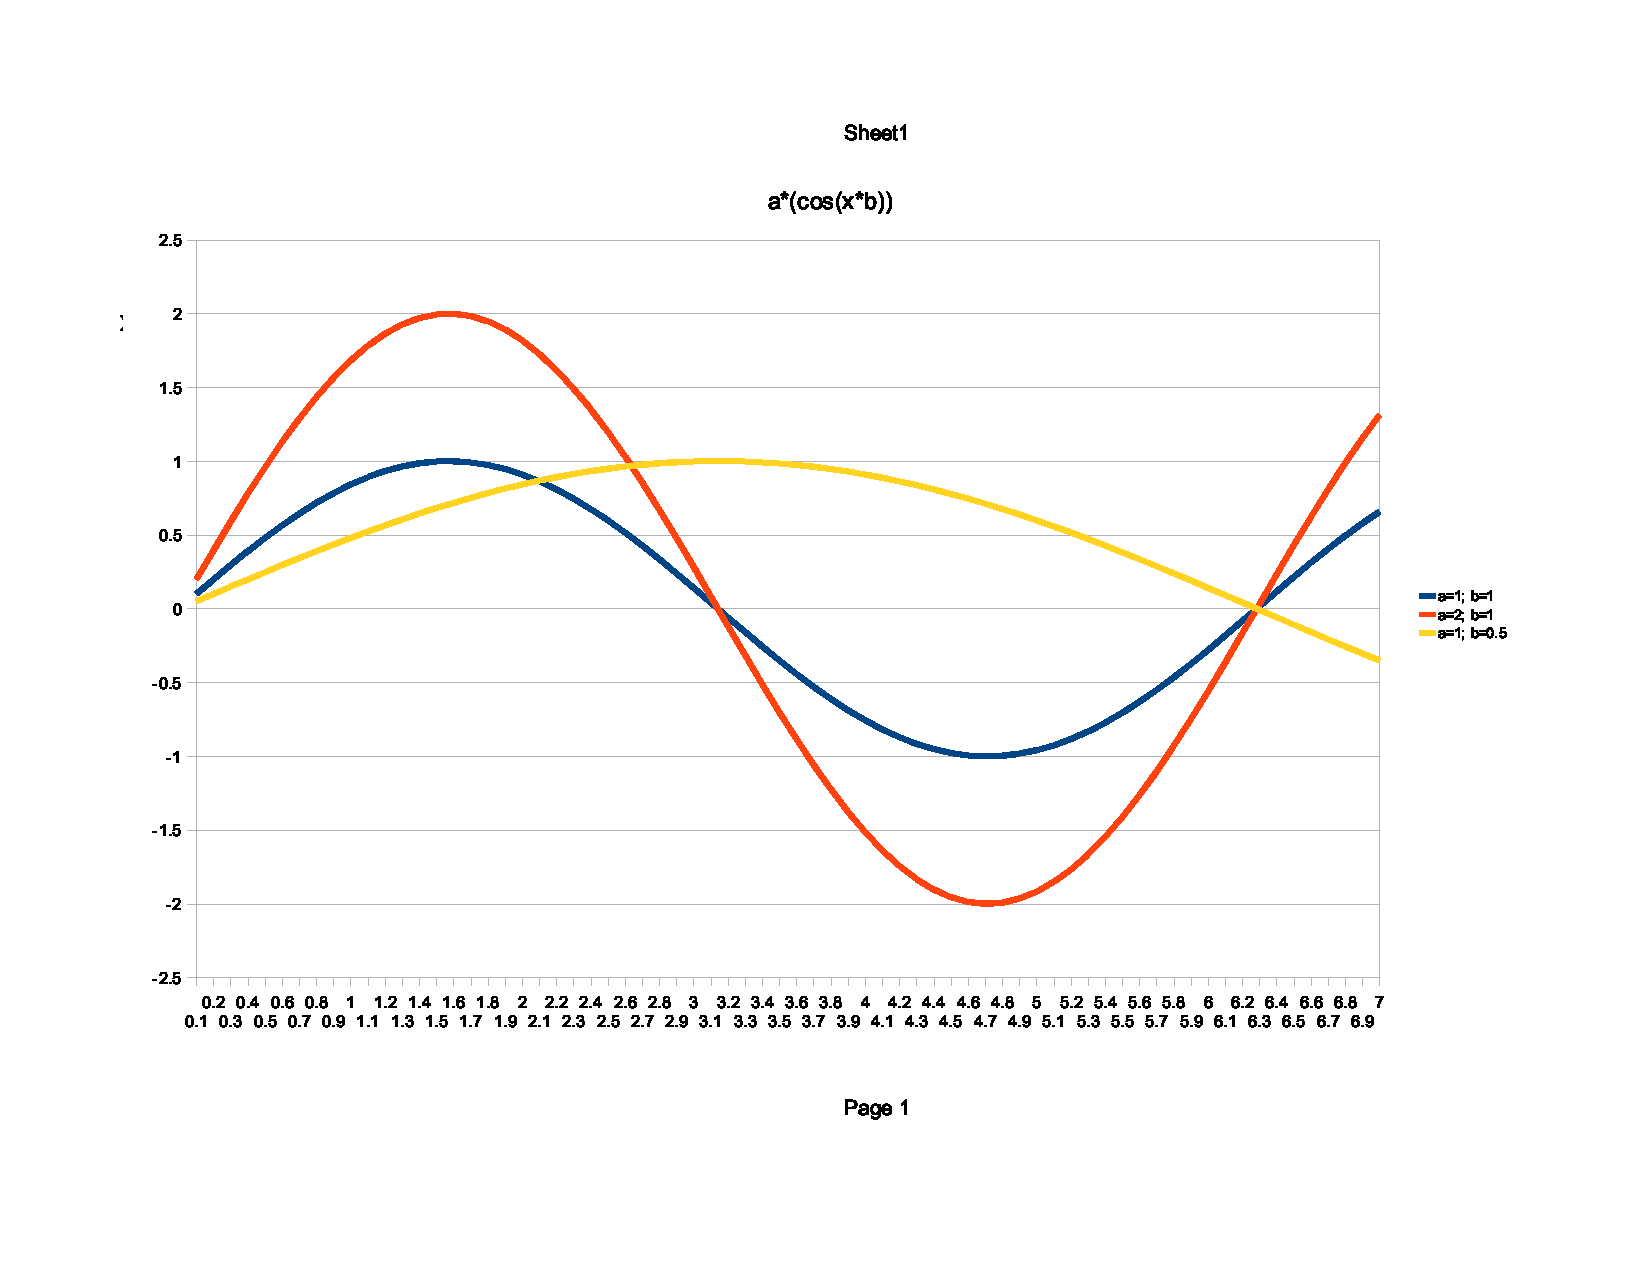
\includegraphics[width=\textwidth]{images/food_function_a}
\caption{Food Function A}
\label{fig:food_function_a}
\end{figure}
Formula b (see figure \vref{fig:food_function_b}) has a skew to the right. I.e.
it increases "slowly" two some point from which on it falls very abruptly. 
\begin{figure}[htb]
\centering
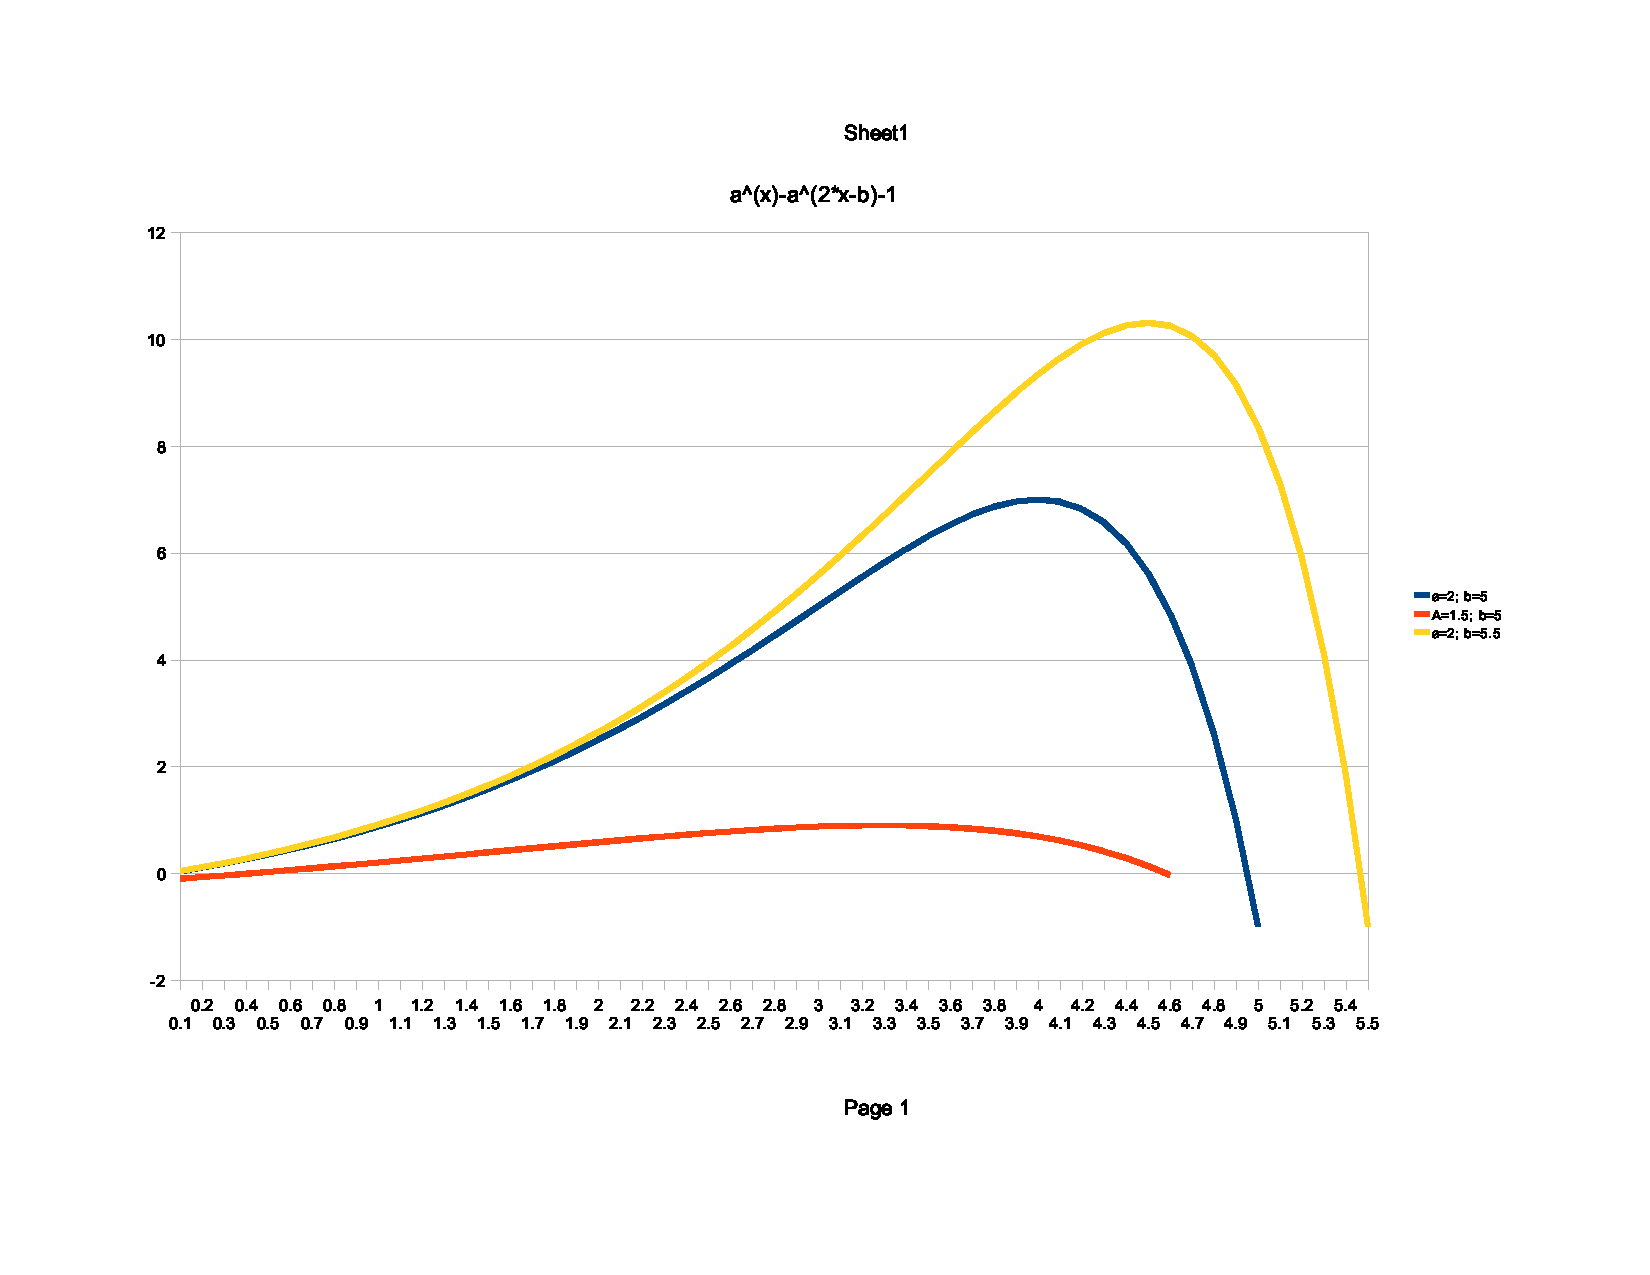
\includegraphics[width=\textwidth]{images/food_function_b}
\caption{Food Function B}
\label{fig:food_function_b}
\end{figure}
These formulas are attached with some sample data as Openoffice spread sheets under attachments.

\paragraph{Implementation}
In order to make it more flexible to choose different algorithms / formulas for
calculating the glucose values the Strategy pattern might be choosen. One
critical question with respect to the implementation is the choice of the used
data types for floatingpoint data as these data types are not guaranteed to be precise.

\subsubsection{Insulin}
\begin{figure}[htb]
\centering
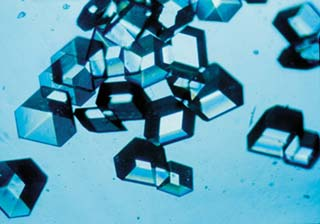
\includegraphics[width=\textwidth]{images/Insulincrystals.jpg}
\caption{Insulin crystals}
\end{figure}
Insulin is a hormone, which is produced in the beta-cells of the pancreas and it's essential for humans and animals. 
Taking of insulin causes decreasing of the blood glucose level and consuming glucagon or energy source. 
Glucagon and some other hormones (e.g. adrenaline, cortisone and pancreas hormones) will increase the blood glucose level.\\
\newpage
In addition some other properties:
\begin{itemize}
  \item after ingestion of carbohydrates the blood glucose level will be increased, 
	  therefore insulin will be degraded to terminate this process
  \item if fats and proteins are eaten at the same time as carbohydrates, 
	  then it will cause delays in absorption of glucose
  \item differences in the absorption speed of glucose between foods with the same amount
  \item movement reduces the need of insulin
\end{itemize}
\newpage
\underline{Types}\\
There are some commonly used types of insulin:\\
\begin{tabular}{lcr}
	\textbf{Synonym} & \textbf{Starts working} & \textbf{Duration}\\
	Insulin analogs (rapid-acting) & 5 to 15 minutes & 3 to 4 hours\\
	Regular insulin(short-acting) & approx. 30 minutes & 5 to 8 hours\\
	Semilente insulin (intermediate-acting) & 1 to 3 hours & 16 to 24 hours\\
	Ultralente insulin (long-acting) & 4 to 6 hours & greater than 32 hours\\
	Insulin glargine/ detemir & 1 to 2 hours & approx. 24 hours\\
	Mixture of NPH and regular insulin & approx. 30 minutes & 16 to 24 hours\\
	Mixture of semilente and ultralente & ? & 24 hours\\
\end{tabular}
\underline{Dosage and Timing}\\
Usually insulin is released into the blood every 3 to 6 minutes. The central problem is to pick the right dose of insulin 
and the right timing. The following diagram shows a plan of the glucose- and insulin levels during the day.\\
\begin{figure}[htb]
\centering
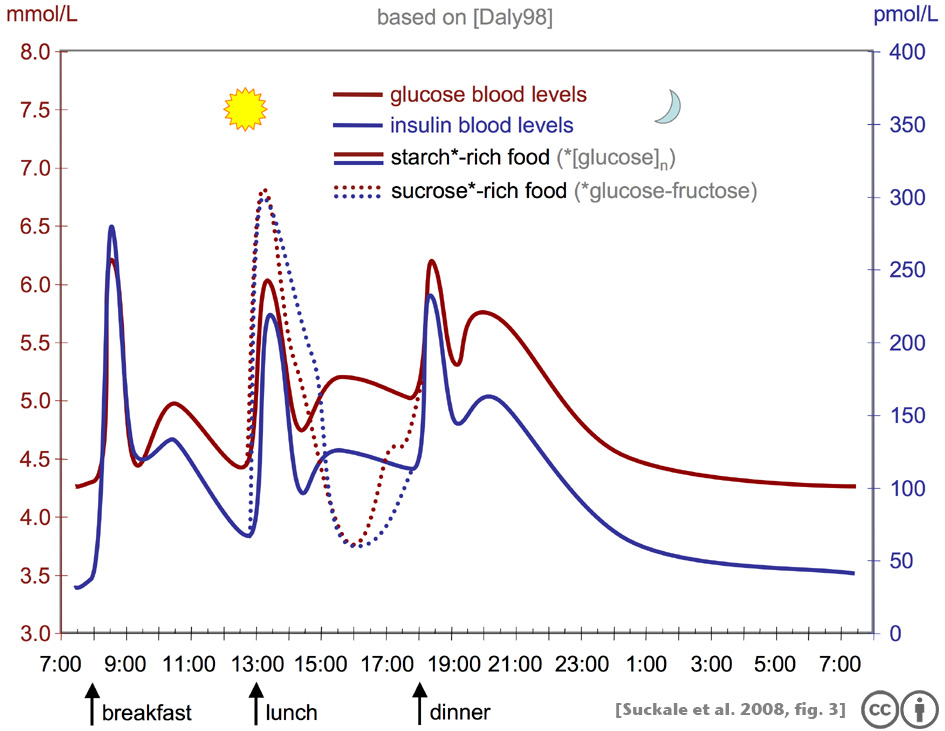
\includegraphics[width=\textwidth]{images/Suckale08_fig3_glucose_insulin_day.jpg}
\caption{Influences of the blood glucose- and insulin level}
\end{figure}
It is impossible to know how much insulin is needed for an optimum blood glucose level, because of the complex and 
interacting factors. For example some patients with diabetes require more insulin after drinking skim milk than 
they do after taking an equivalent amount of fat, protein, carbohydrate, and fluid in some other form.\\
\newpage
\underline{Strategies}:\\
\begin{itemize}
  \item Long-acting insulin will be used for the approximate release of the pancreas (NPH, ultralente, glargine, detemir)
  \item Short-acting insulin will be used for the anticipation of eating (insulin analogs like lispro, aspart and 
	  glulisine can be used while- or after eating, regular insulin has to be used 30 minutes before eating)
  \item The blood glucose level has to be checked before all meals and sometimes also at bedtime
  \item Some guidelines call for check 2 hours after a meal
\end{itemize}
mmol/l <-> mg/dl convertion ; hypoglycemia \& hyperglycemia (Table)\\
\begin{description}
  \item[Red values of blood sugar (hypoglycemia)] The blood sugar is too deep. With progressive drop the blood sugar mirror, the diabetic can fall in coma.
  \item[Green values of blood sugar] Blood sugar within the desirable range. Normal values.
  \item[Turquoise values of blood sugar] The blood sugar is easily increased. (offen after a meal). With a person without diagnosed diabetes further is it necessary to check blood-measurements and to diagnose the diabetes.
  \item[Blue values of blood sugar (hyperglycemia)] Blood sugar values are clearly too high. Non-diabetic should visit the doctor. 
He must be classfy, if he gotten sick. A diabetic must inject immediately fast-effective correction insulin. 
With further blood sugar rising is it possible to get the dangerous coma.
\end{description}
\begin{figure}[htb]
\centering
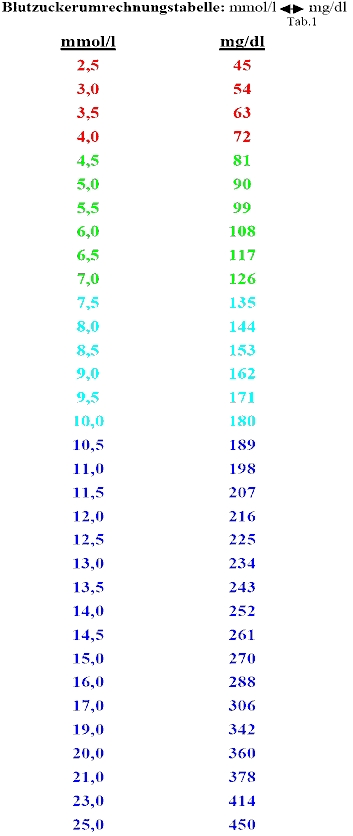
\includegraphics[scale=0.6]{images/Conversion.jpg}
\caption{Blood glucose levels}
\end{figure}
\underline{Existing products}\\
Most insulin products give information about the duration and starting time. The glucose blood level differs from 
human to human, therefore it's difficult to define the effect of the injected insulin. 
Normal blood sugar values are from 4,5 to 7,0 mmol/L and we assume that it's possible to inject max. 12 units insulin 
at once and normally an average of 5 units.\\
\textbf{The effect of one unit insulin?}
\begin{figure}[htb]
\centering
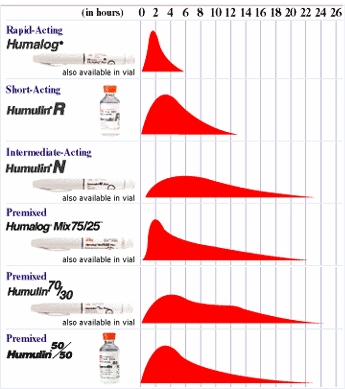
\includegraphics[scale=1]{images/time_activity.jpg}
\caption{Durations of different Canine Insulin types}
\end{figure}

\subsection{Requirements and Project Estimation}
The estimation of the project was done using COCOMO 2.
Therefore the metric used here is Lines Of Code (LOC).

First project estimation:
\begin{itemize}
  \item Behavior Simulation
  	\begin{itemize}
        \item eat (Guess: 450 LOC)
        \item insulin (Guess: 400 LOC)
        \item diabetes (Guess: 400 LOC)
    \end{itemize}
  \item Simulating Insulin Pump
  	\begin{itemize}
        \item actor (Insulin injection) (Guess: 600 LOC)
        \item sensor (Glucose Level Monitor) (Guess: 150 LOC)
        \item User Interface (Alarm/Input) (Guess: 500)
    \end{itemize}
\end{itemize} 
Guessed Estimation based on Experts Cocomo 2:
Effort 13.4 Person-months
Schedule 8.5 Months
\url{http://sunset.usc.edu/cgi-bin/expert_cocomo2000}
